\section{Background}
\label{sec:background}

In this section, we first introduce the preliminary knowledge about electroencephalography (EEG). Then we briefly describe the differences among medical-use EEG devices, research-use EEG devices, and home-use EEG devices. Lastly, we demonstrate our threat model for the home-use EEG devices we are going to investigate. 

\subsection{Background Knowledge of Electroencephalography}
Human brain consists of thousands of nerve cells, also known as neurons. These neurons are constantly receiving, processing, and propagating information through electrical or chemical signals. The neurons are densely interconnected via a nervous structure with numerous synapses serving as intermediaries for passing or inhibiting electrical or chemical signals from one neuron to another neuron. There are two types of synapses: chemical synapse and electrical synapse. A chemical synapse converts an electrical activity from the pre-synaptic neuron into a chemical substance called neurotransmitter which is passed to the post-synaptic cell. Different from the chemical synaptic system, in the electrical synaptic system, the pre-synaptic neuron passes an electrical activity to the post-synaptic neuron through a special channel called gap junction where the electrical activity is converted into an ionic current and therefore inducing voltage changes between the pre-synaptic cell and the post-synaptic cell. Note that electrical synapses transmit signals much more rapidly than chemical synapses, and some synapses can act as both an electrical and a chemical synapse. Electroencephalography (EEG) is an electrophysiological method to detect and monitor the electrical activities of the generated voltages in the electrical synaptic system. Even though the electrical current generated by a single synaptic activity may be too tiny to be detected, fortunately, any human cerebral activity such as surprise, alertness, anger, and so on, usually requires more than 1,000 synaptic activities to complete, making EEG recording, which relies on physical measuring with electrodes attached to a scalp, possible. \\
\indent Even though EEG was introduced about 80 years ago~\cite{swartz1998advantages}, its potential is still actively researched nowadays. In clinical contexts, it has already been well known that EEG can help diagnose various focal disorders such as epilepsy, head injury, encephalitis, brain tumor, encephalopathy, memory problems, sleep disorders, stroke, and dementia~\cite{eegdiagnosis}. In recent years, the ability of EEG to predict Alzheimer's disease is triggering more and more attention~\cite{dauwels2010diagnosis}. In application contexts, besides the various games~\cite{coyle2011eeg}, EEG has been actively studied for the fields such as sleep monitoring~\cite{nakamura2017automatic} or even texting~\cite{zhang2017converting}. On one hand, human beings can benefit from advancing technologies on EEG analysis; on the other hand, as one can readily see, if an individual's EEG data is not properly secured, it can cause severe threats to the individual's privacy.

\subsection{Medical-Use, Research-Use and Home-Use EEG}
According to our research, the current EEG methods and their corresponding devices can be classified into three categories based on the uses of EEG: for strict medical use, for research use, and for home use.

\subsubsection{Strict Medical-Use EEG}
The first type of EEG is intended for strict medical-use, which is mainly employed for focal diagnosis. The EEG data collected for this purpose usually have high dimensions of features. For example, traditional devices such as the large array magnetoencephalography system (MEG) employed by typical hospitals, has up to 125 electrodes attached to a patient's scalp for EEG data collection, which implies that each sample of the EEG data has at least 125 dimensions of features~\cite{lantz2003epileptic}. Since these types of devices are intended for the extreme professional use only, they are usually not available in the open markets for purchase.

\subsubsection{Research-Use EEG}
This type of EEG is intended mainly for research use, e.g., BCI research, which is often considered as a result of downsampling the strict medical-use EEG. One of the most well-known research-use EEG systems is the BCI2000~\cite{schalk2004bci2000}. BCI2000 is a general purpose software system for brain-computer interface research whose device uses 64 electrodes covering a scalp to monitor EEG, which means that each collected data sample has at least 64 features. %The graph of the electrode positions of a BCI2000 device is shown in figure~\ref{fig:bci2000_pos}. 
Even though BCI2000 devices are not intended for strict medical use, they are still classified as professional devices which are costly and are not available for purchase in an open market. A similar system is EPOC~\cite{stytsenko2011evaluation} whose device has 14 electrodes attached to a scalp. This device again is not available for purchase in the markets. %The graph of the electrode positions of an EPOC device is shown in figure~\ref{fig:epoc_pos}.

\subsubsection{Home-Use EEG}
Home-use EEG is intended mainly for home-use applications, i.e., for lightweight medical-related uses. The device of this type of EEG only has three electrodes, with one attached to a person's left earlobe, one attached to the person's left forehead, and the last one attached to the person's right temple. %The graph of electrode positions of a home-use EEG device is shown in figure~ \ref{fig:homeuse_pos}. 
The market of this type of EEG is dominated by a company called NeuroSky~\cite{NeuroSky}, which is the first company to commercialize home-use EEG devices and maintains the largest home-use EEG market share so far~\cite{firsthomeeeg,neuroskymarket}. NeuroSky invented the PCB module, i.e., the ThinkGear AM (TGAM), which serves as a multi-mode sensor to collect EEG data, and the  EEG system framework for EEG data transmission. NeuroSky has an App store where users can purchase or download BCI apps. It also provides a software development kit (SDK) for developers to build BCI apps. All in all, NeuroSky establishes a mature platform for commercialization of the home-use EEG, and hence becomes the most popular brands in home-use EEG. Even though there exist other manufacturers for home-use EEG devices, most of their products leverage TGAM and adopt the EEG system framework. Compared with the previous two types of EEG devices, home-use EEG devices are much more affordable and are publicly available in many online markets such as Amazon. \\
\indent TGAM measures and offers 10 features of EEG, namely attention meter, mediation meter, delta, theta, low alpha, high alpha, low beta, high beta, low gamma, and high gamma. Besides attention meter and mediation meter which are calculated by previously studied algorithms, the other 8 types of the data are traditional EEG waveforms that can be directly measured through different frequencies.
%
\begin{itemize}
  \item \textbf{Delta:} Delta is measured with frequency less than 4 Hz. It is often found during sleeping.
  
  \item \textbf{Theta:} Theta is measured with frequency ranging from 4 Hz to 7 Hz. It is often found during relaxation and meditation.
  
  \item \textbf{Alpha:} There are two types of alpha: low alpha which is measured with frequency ranging from 8 Hz to 9 Hz and high alpha which is measured with frequency ranging from 10 Hz to 12 Hz. Alpha is usually detected when eyes are closed or during relaxation.
  
  \item \textbf{Beta:} There are two types of beta: low beta which is measured with frequency ranging from 13 Hz to 17 Hz and high beta which is measured with frequency ranging from 18 Hz to 30 Hz. Beta is usually found during alertness or focuses. 
  
  \item \textbf{Gamma:} There are two types of gamma: low gamma which is measured with frequency ranging from 31 Hz to 40 Hz and high gamma which is measured with frequency ranging from 41 Hz to 50 Hz. Gamma is usually associated with multi-sensory processing, e.g., perception involving different senses such as sound and sight. 
\end{itemize}

Note that NeuroSky produces two types of EEG headsets: one is intended for personal computer (PC) only and the other can be used for both PC and mobile devices such as Android and iOS. However, we notice that the headset intended for PC only is much more popular than the one intended for both PC and mobiles since the purchase number of the former far exceeds the latter both on Amazon and Google Shop, and all the 156 apps on the NeuroSky official App store have a PC version but only 45 (25.85\%) of them have the mobile version. On the other hand, the mechanism adopted by the mobiles is basically the same as the one adopted by PC. Therefore, in this paper, we conducted all our analysis against the PC platform since it is more meaningful.
  
\subsection{Threat Model}
In our adversarial model, attackers aim to steal brain waves of NeuroSky users and infer sensitive personal activity from these brain waves. For our remote attacks, we assume that an adversary is able to install a malicious program into a victim's PC and to execute the malicious program. There exist various ways for the adversary to accomplish this task. For example, the adversary can perform social engineering~\cite{socialengineering}, or exploit the known remote code execution (RCE) vulnerabilities~\cite{rce} and advanced persistent threat (APT)~\cite{apt}. Note that these techniques are all viable and feasible, and have been widely adopted as attack vectors for compromising industrial systems~\cite{socialengieerstat}\cite{aptstat}\cite{vulstat}. In this paper, we do not detail these procedures since they are out of the scope of this research. On the other hand, our proximate attack requires an adversary to be in a short-distance range, i.e., no more than 22 meters, away from the victim. However, the adversary does not need to have any access to any of the victim's devices. An adversary exploiting this attack can be a malicious neighbor, or a stalker who approaches the victim's home. If the victim wears the EEG headset device in a public area along with his laptop, the adversary can simply launch the attack in a nearby area, which could be some distance away and blocked by a few layers of walls, without triggering his suspicion. The adversary only needs to purchase related devices such as a GNU radio for a few hundred dollars.

%\begin{figure*}[h]
%        %\quad
%        \begin{subfigure}[t]{0.33\textwidth}
%          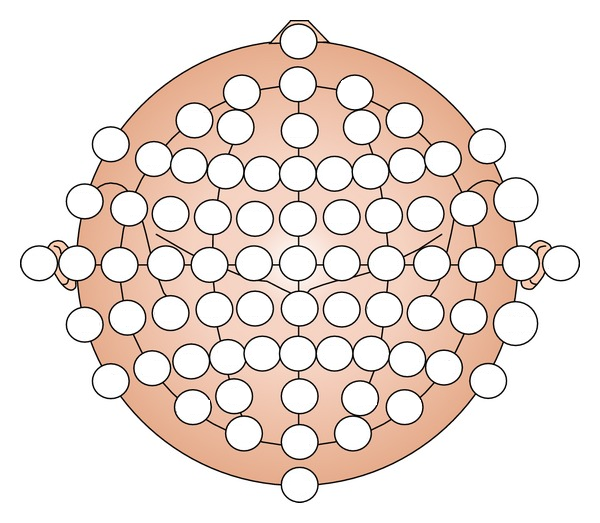
\includegraphics[width=0.975\linewidth]{bci2000_position.png}
%                \caption{BCI2000 device}
%                \label{fig:bci2000_pos}
%        \end{subfigure}
%        \begin{subfigure}[t]{0.33\textwidth}
%         \centering
%          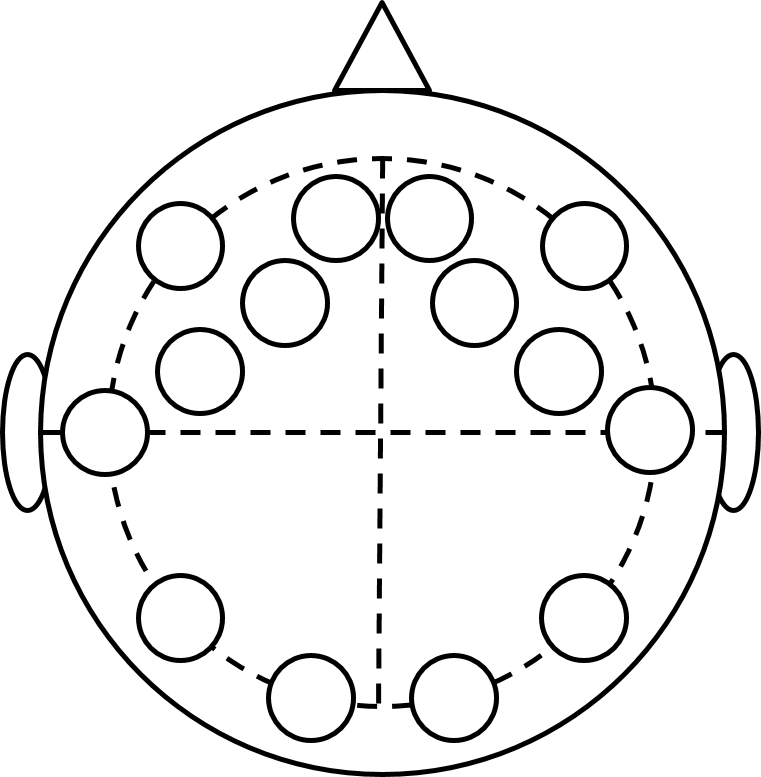
\includegraphics[width=0.8\linewidth]{epoc_position.png}
%                \caption{EPOC devices}
%                \label{fig:epoc_pos}
%        \end{subfigure}%
%        %\quad
%        \begin{subfigure}[t]{0.33\textwidth}
%          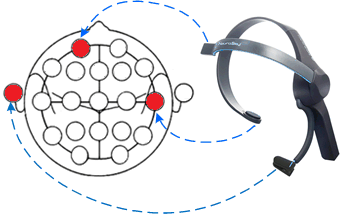
\includegraphics[width=0.975\linewidth, height=0.7\linewidth]{neurosky_position.jpg}
%                \caption{Home-Use EEG device}
%                \label{fig:homeuse_pos}
%        \end{subfigure}
%         \caption{Electrode positions in a human scalp of the EEG devices. A BCI2000 device has 64 electrodes, an EPOC device has 14 electrodes, while a home-use EEG device has only 3 electrodes.}
%         \label{fig:electrodepos}
%\end{figure*}
